%===========================================================
% 10_teamwork.tex - 团队协作开发实战
%===========================================================

\section{Git工作流实践}

\begin{frame}{分支策略:Git Flow}
    \begin{center}
        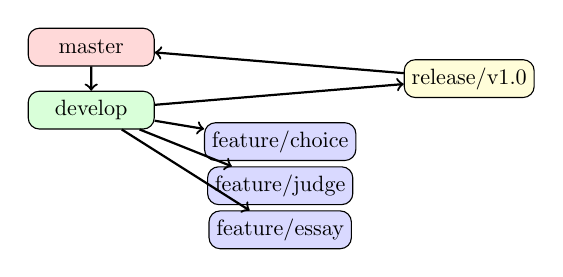
\begin{tikzpicture}[scale=0.8, transform shape,
            box/.style={draw, rectangle, rounded corners, fill=blue!15, minimum width=2cm, minimum height=0.6cm, align=center},
            main/.style={draw, rectangle, rounded corners, fill=red!15, minimum width=2cm, minimum height=0.6cm, align=center},
            develop/.style={draw, rectangle, rounded corners, fill=green!15, minimum width=2cm, minimum height=0.6cm, align=center}]

            % 主分支
            \node[main] (master) at (0,0) {master};
            \node[develop] (dev) at (0,-1) {develop};

            % 功能分支
            \node[box] (f1) at (3,-1.5) {feature/choice};
            \node[box] (f2) at (3,-2.2) {feature/judge};
            \node[box] (f3) at (3,-2.9) {feature/essay};

            % 发布分支
            \node[box, fill=yellow!15] (rel) at (6,-0.5) {release/v1.0};

            % 连接
            \draw[->, thick] (master) -- (dev);
            \draw[->, thick] (dev) -- (f1);
            \draw[->, thick] (dev) -- (f2);
            \draw[->, thick] (dev) -- (f3);
            \draw[->, thick] (dev) -- (rel);
            \draw[->, thick] (rel) -- (master);
        \end{tikzpicture}
    \end{center}

    \vspace{0.3cm}

    \textbf{分支说明:}
    \begin{itemize}
        \item \textbf{master}:生产分支,只接受合并
        \item \textbf{develop}:开发分支,功能集成
        \item \textbf{feature/*}:功能分支,从develop创建
        \item \textbf{release/*}:发布分支,准备上线
        \item \textbf{hotfix/*}:紧急修复,从master创建
    \end{itemize}
\end{frame}

\begin{frame}{GitHub Flow简化工作流}
    \textbf{适合小团队的简化流程:}

    \vspace{0.3cm}

    \begin{enumerate}
        \item \textbf{主分支保护}:master分支受保护
        \item \textbf{功能分支开发}:从master创建feature分支
        \item \textbf{提交Pull Request}:完成功能后提交PR
        \item \textbf{代码审查}:至少1人review通过
        \item \textbf{合并到主分支}:CI通过后合并
        \item \textbf{删除功能分支}:保持仓库整洁
    \end{enumerate}

    \vspace{0.3cm}

    \begin{lstlisting}
# 1. 创建功能分支
git checkout -b feature/choice-recognizer

# 2. 开发和提交
git add .
git commit -m "实现选择题识别器"

# 3. 推送到远程
git push origin feature/choice-recognizer

# 4. 在GitHub上创建Pull Request
# 5. 代码审查后合并
    \end{lstlisting}
\end{frame}

\begin{frame}{代码审查流程}
    \begin{block}{代码审查(Code Review)原则}
        \begin{itemize}
            \item 所有代码必须经过review才能合并
            \item 审查关注:功能、性能、安全、风格
            \item 提出问题要具体,给出改进建议
            \item 保持尊重,对代码不对人
        \end{itemize}
    \end{block}

    \vspace{0.3cm}

    \textbf{审查清单:}
    \begin{table}
        \centering
        \small
        \begin{tabular}{p{2cm}p{8cm}}
            \toprule
            \textbf{检查项} & \textbf{内容} \\
            \midrule
            功能性 & 代码是否实现了需求?边界条件处理了吗? \\
            可读性 & 命名是否清晰?注释是否充分? \\
            可维护性 & 是否遵循设计原则?是否高内聚低耦合? \\
            性能 & 是否有明显性能问题?算法复杂度如何? \\
            安全性 & 是否有注入风险?敏感信息处理? \\
            \bottomrule
        \end{tabular}
    \end{table}
\end{frame}

\begin{frame}{冲突解决与合并}
    \begin{block}{避免冲突的最佳实践}
        \begin{itemize}
            \item 频繁提交,小步迭代
            \item 开发前先从主分支拉取最新代码
            \item 不要长时间在分支上开发
            \item 与团队成员沟通,避免同时修改同一文件
        \end{itemize}
    \end{block}

    \vspace{0.3cm}

    \textbf{解决冲突步骤:}
    \begin{lstlisting}
# 1. 拉取最新代码
git pull origin develop

# 2. 如果有冲突,会提示冲突文件
# 打开冲突文件,找到 <<<<<<< ======= >>>>>>> 标记

# 3. 手动编辑,保留需要的代码

# 4. 标记冲突已解决
git add <冲突文件>

# 5. 提交合并
git commit -m "合并develop分支,解决冲突"
    \end{lstlisting}
\end{frame}

\begin{frame}{版本发布管理}
    \textbf{语义化版本(Semantic Versioning):}

    \begin{center}
        \Large \textbf{MAJOR.MINOR.PATCH}
    \end{center}

    \begin{itemize}
        \item \textbf{MAJOR}:不兼容的API修改
        \item \textbf{MINOR}:向下兼容的功能新增
        \item \textbf{PATCH}:向下兼容的问题修复
    \end{itemize}

    \vspace{0.3cm}

    \begin{lstlisting}
# 创建版本标签
git tag -a v1.0.0 -m "第一个正式版本"
git push origin v1.0.0

# 查看标签
git tag

# 切换到某个版本
git checkout v1.0.0
    \end{lstlisting}

    \begin{exampleblock}{版本示例}
        v0.1.0(内测版)→ v0.9.0(公测版)→ v1.0.0(正式版)→ v1.1.0(功能更新)
    \end{exampleblock}
\end{frame}

\section{代码规范与文档}

\begin{frame}{PEP 8代码规范}
    \textbf{命名规范:}
    \begin{table}
        \centering
        \small
        \begin{tabular}{p{2.5cm}p{3cm}p{4.5cm}}
            \toprule
            \textbf{类型} & \textbf{规范} & \textbf{示例} \\
            \midrule
            模块/包 & 小写,短名称 & \texttt{recognition}, \texttt{utils} \\
            类 & 驼峰命名 & \texttt{ChoiceRecognizer} \\
            函数/方法 & 小写下划线 & \texttt{recognize\_choice()} \\
            常量 & 大写下划线 & \texttt{MAX\_IMAGE\_SIZE} \\
            私有变量 & 前导下划线 & \texttt{\_internal\_data} \\
            \bottomrule
        \end{tabular}
    \end{table}

    \vspace{0.3cm}

    \textbf{代码布局:}
    \begin{itemize}
        \item 缩进:4个空格(禁用Tab)
        \item 行宽:最大79字符
        \item 空行:顶级函数/类间2行,方法间1行
        \item 导入:标准库→第三方→本地,每组空一行
    \end{itemize}
\end{frame}

\begin{frame}{类型注解与文档字符串}
    \begin{lstlisting}
from typing import List, Optional, Dict
import numpy as np

def recognize_choices(
    image: np.ndarray,
    regions: List[tuple],
    threshold: float = 0.5
) -> Dict[str, str]:
    """识别选择题答案

    Args:
        image: 输入图像,BGR格式
        regions: 选项区域列表 [(x, y, w, h), ...]
        threshold: 填涂检测阈值,默认0.5

    Returns:
        字典,键为题号,值为答案(A/B/C/D)

    Raises:
        ValueError: 图像格式不正确

    Example:
        >>> result = recognize_choices(img, [(10, 10, 50, 20)])
        >>> print(result)
        {'1': 'A', '2': 'B'}
    """
    # 实现代码...
    pass
    \end{lstlisting}
\end{frame}

\begin{frame}{接口文档生成}
    \textbf{使用工具自动生成文档:}

    \vspace{0.3cm}

    \begin{columns}
        \column{0.5\textwidth}
        \textbf{Sphinx:}
        \begin{itemize}
            \item Python标准文档工具
            \item 支持reStructuredText
            \item 生成HTML/PDF/ePub
            \item 支持自动生成API文档
        \end{itemize}

        \vspace{0.3cm}

        \textbf{MkDocs:}
        \begin{itemize}
            \item 基于Markdown
            \item 配置简单
            \item 美观的主题
            \item 适合项目文档
        \end{itemize}

        \column{0.5\textwidth}
        \textbf{pdoc:}
        \begin{itemize}
            \item 零配置文档生成
            \item 直接从docstring生成
            \item 支持类型注解
            \item 自动生成导航
        \end{itemize}

        \vspace{0.3cm}

        \begin{lstlisting}
# 安装
pip install pdoc

# 生成文档
pdoc --html mymodule

# 启动文档服务器
pdoc --http : mymodule
        \end{lstlisting}
    \end{columns}
\end{frame}

\section{团队协作实践}

\begin{frame}{任务分配与跟踪}
    \textbf{任务分解原则:}
    \begin{itemize}
        \item 每个任务可独立完成(1-3天)
        \item 任务有明确的验收标准
        \item 任务间依赖关系清晰
        \item 预留缓冲时间应对风险
    \end{itemize}

    \vspace{0.3cm}

    \begin{table}
        \centering
        \small
        \begin{tabular}{p{2cm}p{2cm}p{2cm}p{4cm}}
            \toprule
            \textbf{任务} & \textbf{负责人} & \textbf{截止时间} & \textbf{验收标准} \\
            \midrule
            选择题识别 & 张三 & 第10周 & 准确率>95\%,有单元测试 \\
            判断题识别 & 李四 & 第10周 & 准确率>95\%,有单元测试 \\
            简答题识别 & 王五 & 第11周 & 集成OCR,能识别手写 \\
            评分模块 & 赵六 & 第11周 & 支持多种评分规则 \\
            \bottomrule
        \end{tabular}
    \end{table}
\end{frame}

\begin{frame}{每日站会与进度同步}
    \begin{block}{每日站会(Daily Stand-up)}
        \begin{itemize}
            \item 时间:固定时间,15分钟以内
            \item 形式:站立进行,保持高效
            \item 每人回答三个问题:
                \begin{enumerate}
                    \item 昨天完成了什么?
                    \item 今天计划做什么?
                    \item 有什么阻碍?
                \end{enumerate}
        \end{itemize}
    \end{block}

    \vspace{0.3cm}

    \textbf{进度同步工具:}
    \begin{itemize}
        \item 看板(Kanban):直观展示任务状态
        \item 燃尽图(Burndown):跟踪进度趋势
        \item 甘特图(Gantt):展示任务时间安排
    \end{itemize}
\end{frame}

\begin{frame}{问题沟通与解决}
    \textbf{问题升级路径:}

    \begin{center}
        \begin{tikzpicture}[scale=0.8, transform shape,
            box/.style={draw, rectangle, rounded corners, fill=blue!15, minimum width=3cm, minimum height=0.8cm, align=center}]

            \node[box] (self) at (0,0) {1. 自主解决\\查阅文档、Google};
            \node[box] (team) at (0,-1.5) {2. 团队讨论\\请教组员、技术负责人};
            \node[box] (lead) at (0,-3) {3. 组长介入\\调整方案、协调资源};
            \node[box] (teacher) at (0,-4.5) {4. 求助老师\\技术难点、方向决策};

            \draw[->, thick] (self) -- (team) node[midway, right] {30分钟};
            \draw[->, thick] (team) -- (lead) node[midway, right] {2小时};
            \draw[->, thick] (lead) -- (teacher) node[midway, right] {半天};
        \end{tikzpicture}
    \end{center}

    \vspace{0.3cm}

    \begin{alertblock}{沟通原则}
        遇到问题不要憋太久,及时求助。但同时也要先自己尝试解决,带着思考去提问。
    \end{alertblock}
\end{frame}
